% !TEX program = xelatex
\documentclass[UTF8,fontset=fandol,a4paper,11pt]{ctexart}
\usepackage[margin=21mm,top=23mm,bottom=22mm,headheight=16pt]{geometry}
\usepackage{amsmath,amssymb,mathtools,bm}
\usepackage{tikz}
\usetikzlibrary{arrows.meta,calc,angles,quotes,patterns}
\usepackage{xcolor,booktabs,array,longtable,enumitem,fancyhdr,needspace}
\usepackage[unicode,hidelinks]{hyperref}
\definecolor{ink}{HTML}{24343C}
\definecolor{accent}{HTML}{166A70}
\definecolor{muted}{HTML}{65747A}
\definecolor{rulegray}{HTML}{D4DDE0}
\definecolor{warm}{HTML}{966037}
\color{ink}
\setlength{\parindent}{2em}
\setlength{\parskip}{4pt}
\linespread{1.12}
\AtBeginDocument{\setlength{\abovedisplayskip}{6pt plus 2pt minus 1pt}
\setlength{\belowdisplayskip}{6pt plus 2pt minus 1pt}
\setlength{\abovedisplayshortskip}{0pt plus 1pt}
\setlength{\belowdisplayshortskip}{4pt plus 1pt}}
\setlist[enumerate]{label=(\arabic*),leftmargin=2.3em,itemsep=3pt,topsep=4pt}
\setlist[itemize]{leftmargin=2em,itemsep=2pt,topsep=4pt}
\allowdisplaybreaks[1]
\setlength{\emergencystretch}{2em}
\setcounter{secnumdepth}{0}
\providecommand{\tightlist}{\setlength{\itemsep}{0pt}\setlength{\parskip}{0pt}}
\ctexset{section={format=\Large\bfseries\color{accent},beforeskip=10pt,afterskip=9pt},
subsection={format=\normalsize\bfseries\color{accent},beforeskip=10pt,afterskip=4pt},
subsubsection={format=\normalsize\bfseries,beforeskip=8pt,afterskip=3pt}}
\pagestyle{fancy}
\fancyhf{}
\fancyhead[L]{\small\color{muted}物理学难题集萃}
% 页眉仅保留书名；版本名称只在封面显示。
\fancyfoot[L]{\small\color{muted}\chapterlabel}
\fancyfoot[R]{\small\thepage}
\renewcommand{\headrulewidth}{0.4pt}
\renewcommand{\footrulewidth}{0pt}
\newcommand{\dd}{\mathop{}\!\mathrm{d}}
\newcommand{\vect}[1]{\bm{#1}}
\newcommand{\tagline}[1]{\noindent{\small\color{muted}#1}\par}
\newcommand{\result}[1]{\begin{equation*}\boxed{#1}\end{equation*}}
\newcommand{\figcaption}[1]{\par\vspace{2pt}{\small\color{muted}#1}\par}
\newcommand{\teach}[2]{\Needspace{4\baselineskip}\subsection*{讲解要点与追问}#1\par\smallskip\noindent\textbf{追问：}#2\par}
\newcommand{\workarea}{\par\vspace{7mm}\noindent{\small\color{muted}作答区}\par\vspace{4mm}
\noindent\textcolor{rulegray}{\rule{\linewidth}{0.3pt}}\par\vspace{16mm}
\noindent\textcolor{rulegray}{\rule{\linewidth}{0.3pt}}\par\vspace{16mm}
\noindent\textcolor{rulegray}{\rule{\linewidth}{0.3pt}}\par\vspace{16mm}
\noindent\textcolor{rulegray}{\rule{\linewidth}{0.3pt}}}
\tikzset{axis/.style={-{Stealth[length=2mm]},thin,color=muted},
motion/.style={-{Stealth[length=2.3mm]},thick,color=accent},
force/.style={-{Stealth[length=2.3mm]},thick,color=warm},
traj/.style={thick,color=accent},guide/.style={dashed,thin,color=muted},
object/.style={thick,color=ink},every node/.style={font=\small}}\widowpenalty=10000\clubpenalty=10000\displaywidowpenalty=10000\newcommand{\chapterlabel}{光学第四章\quad 光的偏振}







\hypersetup{pdftitle={光学第四章 光的偏振·学生版},pdfauthor={}}

\begin{document}\pdfbookmark[0]{光学第四章 光的偏振}{cover}

\thispagestyle{empty}\vspace*{22mm}

\noindent{\Huge\bfseries 物理学难题集萃}\par\vspace{10mm}

\noindent{\LARGE 光学第四章}\par\vspace{6mm}

\noindent{\LARGE 光的偏振}\par\vspace{12mm}

\noindent{\Large\color{accent}学生版}\par\vspace{9mm}

\noindent\textcolor{accent}{\rule{\linewidth}{1pt}}\par\vspace{9mm}

\noindent 第1--35题\par\vfill\clearpage

\pdfbookmark[1]{题目目录}{contents}\section*{题目目录}

\begin{longtable}{@{}r p{113mm} r@{}}\toprule 题号 & 题目 & 页码\\\midrule

\hyperref[q:1]{1} & \hyperref[q:1]{自然光通过理想偏振片} & \pageref{q:1} \\

\hyperref[q:2]{2} & \hyperref[q:2]{旋转检偏器与部分偏振光} & \pageref{q:2} \\

\hyperref[q:3]{3} & \hyperref[q:3]{多层膜偏振分束棱镜} & \pageref{q:3} \\

\hyperref[q:4]{4} & \hyperref[q:4]{反射与折射后的偏振方向} & \pageref{q:4} \\

\hyperref[q:5]{5} & \hyperref[q:5]{斜反射自然光的偏振度} & \pageref{q:5} \\

\hyperref[q:6]{6} & \hyperref[q:6]{布儒斯特入射的振幅、强度与功率} & \pageref{q:6} \\

\hyperref[q:7]{7} & \hyperref[q:7]{玻璃片堆的偏振选择} & \pageref{q:7} \\

\hyperref[q:8]{8} & \hyperref[q:8]{全反射引入的相位差} & \pageref{q:8} \\

\hyperref[q:9]{9} & \hyperref[q:9]{由椭偏反射比求折射率} & \pageref{q:9} \\

\hyperref[q:10]{10} & \hyperref[q:10]{石英棱镜的双折射分离} & \pageref{q:10} \\

\hyperref[q:11]{11} & \hyperref[q:11]{用已知波片识别未知波片的快轴} & \pageref{q:11} \\

\hyperref[q:12]{12} & \hyperref[q:12]{用圆偏振光标定方解石快轴} & \pageref{q:12} \\

\hyperref[q:13]{13} & \hyperref[q:13]{两次检偏强度与偏振度} & \pageref{q:13} \\

\hyperref[q:14]{14} & \hyperref[q:14]{圆偏振经波片后的检偏强度} & \pageref{q:14} \\

\hyperref[q:15]{15} & \hyperref[q:15]{两只圆偏振器的排列与轴向} & \pageref{q:15} \\

\hyperref[q:16]{16} & \hyperref[q:16]{偏振片与波片抑制镜面回光} & \pageref{q:16} \\

\hyperref[q:17]{17} & \hyperref[q:17]{椭圆偏振光的检偏极值与主轴} & \pageref{q:17} \\

\hyperref[q:18]{18} & \hyperref[q:18]{旋向不同的椭偏光通过延迟片} & \pageref{q:18} \\

\hyperref[q:19]{19} & \hyperref[q:19]{部分椭偏光的自然分量} & \pageref{q:19} \\

\hyperref[q:20]{20} & \hyperref[q:20]{波片产生椭圆偏振的主轴与轴比} & \pageref{q:20} \\

\hyperref[q:21]{21} & \hyperref[q:21]{双孔干涉中的偏振标记与检偏} & \pageref{q:21} \\

\hyperref[q:22]{22} & \hyperref[q:22]{正交晶轴双片改变双孔条纹} & \pageref{q:22} \\

\hyperref[q:23]{23} & \hyperref[q:23]{两片串联产生可调线偏方向} & \pageref{q:23} \\

\hyperref[q:24]{24} & \hyperref[q:24]{白光波片的消光波长} & \pageref{q:24} \\

\hyperref[q:25]{25} & \hyperref[q:25]{双折射劈尖的偏振干涉条纹} & \pageref{q:25} \\

\hyperref[q:26]{26} & \hyperref[q:26]{非共线异旋圆偏振的电场干涉} & \pageref{q:26} \\

\hyperref[q:27]{27} & \hyperref[q:27]{单臂晶片对圆偏双孔条纹的作用} & \pageref{q:27} \\

\hyperref[q:28]{28} & \hyperref[q:28]{克尔盒的电压调制与条纹可见度} & \pageref{q:28} \\

\hyperref[q:29]{29} & \hyperref[q:29]{旋光石英棱镜的圆双折射角分离} & \pageref{q:29} \\

\hyperref[q:30]{30} & \hyperref[q:30]{尼科耳棱镜的角视场} & \pageref{q:30} \\

\hyperref[q:31]{31} & \hyperref[q:31]{波法线与能流方向的最大走离角} & \pageref{q:31} \\

\hyperref[q:32]{32} & \hyperref[q:32]{各向同性介质向晶体的全反射条件} & \pageref{q:32} \\

\hyperref[q:33]{33} & \hyperref[q:33]{晶体内反射的光线角关系} & \pageref{q:33} \\

\hyperref[q:34]{34} & \hyperref[q:34]{晶体界面的振幅反射与透射} & \pageref{q:34} \\

\hyperref[q:35]{35} & \hyperref[q:35]{晶体界面的可逆路径与斯托克斯关系} & \pageref{q:35} \\

\bottomrule\end{longtable}

\clearpage

\pdfbookmark[2]{第 1 题 自然光通过理想偏振片}{q1}

\section*{第 1 题\quad 自然光通过理想偏振片}\label{q:1}

自然光垂直入射理想线偏振片。证明透射光强为入射光强的一半，并说明为什么偏振片转动时结果不变。

\begin{center}\begin{minipage}{.98\linewidth}\centering
\begin{tikzpicture}[scale=.9,transform shape]
\draw[axis] (-1.60000,0.00000)--(1.60000,0.00000);\draw[axis] (0.00000,-1.60000)--(0.00000,1.60000);\node[below right] at (1.60000,0.00000) {$x$};\node[above right] at (0.00000,1.60000) {$y$};\draw[force] (-1.35946,-0.63393)--(1.35946,0.63393);\node[above right] at (1.47728,0.68887) {$\boldsymbol p$};\draw[thin,color=muted] (-1.05000,0.00000)--(1.05000,0.00000);\draw[thin,color=muted] (-0.98668,-0.35912)--(0.98668,0.35912);\draw[thin,color=muted] (-0.80435,-0.67493)--(0.80435,0.67493);\draw[thin,color=muted] (-0.52500,-0.90933)--(0.52500,0.90933);\draw[thin,color=muted] (-0.18233,-1.03405)--(0.18233,1.03405);\draw[thin,color=muted] (0.18233,-1.03405)--(-0.18233,1.03405);\draw[thin,color=muted] (0.52500,-0.90933)--(-0.52500,0.90933);\draw[thin,color=muted] (0.80435,-0.67493)--(-0.80435,0.67493);\draw[thin,color=muted] (0.98668,-0.35912)--(-0.98668,0.35912);\node[above] at (0.00000,2.20000) {自然光：横向无优先方向};
\end{tikzpicture}
\figcaption{图光4.1\quad 横截面上的自然光与透光轴}
\end{minipage}\end{center}

\workarea

\clearpage

\pdfbookmark[2]{第 2 题 旋转检偏器与部分偏振光}{q2}

\section*{第 2 题\quad 旋转检偏器与部分偏振光}\label{q:2}

任意一束部分偏振光通过理想线检偏器，转动检偏器一周。求透射强度随方位角的通式，说明最大、最小透射方向的关系，并证明：就线检偏器的透射结果而言，该光束可等效为自然光与线偏振光的叠加。讨论透射强度与角度无关的情况。

\begin{center}\begin{minipage}{.98\linewidth}\centering
\begin{tikzpicture}[scale=.9,transform shape]
\draw[motion] (-1.00000,0.00000)--(1.00000,0.00000);\draw[object] (-0.12000,-0.80000)--(0.12000,-0.80000)--(0.12000,0.80000)--(-0.12000,0.80000)--(-0.12000,-0.80000);\node[above] at (0.00000,1.00000) {检偏器};\node[below] at (0.00000,-1.05000) {$\theta$};\begin{scope}[shift={(4.00000,0.00000)}]
\draw[axis] (-1.60000,0.00000)--(1.60000,0.00000);\draw[axis] (0.00000,-1.60000)--(0.00000,1.60000);\node[below right] at (1.60000,0.00000) {$x$};\node[above right] at (0.00000,1.60000) {$y$};\draw[force] (-1.22873,-0.86036)--(1.22873,0.86036);\node[above right] at (1.33522,0.93493) {$\theta$};
\end{scope}
\end{tikzpicture}
\figcaption{图光4.2\quad 检偏器角度相对于固定入射横轴定义}
\end{minipage}\end{center}

\workarea

\clearpage

\pdfbookmark[2]{第 3 题 多层膜偏振分束棱镜}{q3}

\section*{第 3 题\quad 多层膜偏振分束棱镜}\label{q:3}

偏振分束立方体由两块相同直角棱镜胶合构成，平行光垂直入射外表面，在斜面处的棱镜内入射角为$45^\circ$。胶合面镀交替的高、低折射率膜，$n_H=2.38,n_L=1.25$，工作波长为$514.5\,\mathrm{nm}$。求使膜层内部各界面对$p$偏振满足布儒斯特条件的棱镜折射率，以及使$s$反射相长的最小正膜厚。说明有限膜系实现分束还需要哪些条件。忽略色散、吸收与胶层厚度。

\begin{center}\begin{minipage}{.98\linewidth}\centering
\begin{tikzpicture}[scale=.9,transform shape]
\draw[motion] (-1.20000,2.70000)--(0.00000,1.50000);
\draw[motion] (0.00000,1.50000)--(-1.20000,0.30000);\draw[force] (0.00000,1.50000)--(0.25000,1.36870);
\draw[force] (0.25000,1.36870)--(1.15630,-0.35691);
\draw[force] (1.15630,-0.35691)--(2.65630,-1.85691);\draw[thin] (0.00000,-2.00000)--(0.00000,2.00000);\draw[thin] (0.25000,-2.00000)--(0.25000,2.00000);\draw[thin] (1.15630,-2.00000)--(1.15630,2.00000);\node[below] at (0.12500,-2.20000) {$H$};\node[below] at (0.70315,-2.20000) {$L$};\node[above] at (1.50000,3.10000) {一对$HL$膜；可继续成对叠加};\node[left] at (-1.00000,-1.00000) {棱镜 $n$};\node[right] at (3.00000,-1.80000) {棱镜 $n$};
\end{tikzpicture}
\figcaption{图光4.3\quad 偏振分束的高低折射率交替膜}
\end{minipage}\end{center}

\workarea

\clearpage

\pdfbookmark[2]{第 4 题 反射与折射后的偏振方向}{q4}

\section*{第 4 题\quad 反射与折射后的偏振方向}\label{q:4}

线偏振光从折射率$n_1$的透明介质射向折射率$n_2$的透明介质，入射角为$\theta_1$，电矢量与入射面夹角为$\alpha$。求反射光、折射光的偏振方向，并讨论布儒斯特入射、法向入射及全反射。

\begin{center}\begin{minipage}{.98\linewidth}\centering
\begin{tikzpicture}[scale=.9,transform shape]
\draw[object] (-3.10000,0.00000)--(3.50000,0.00000);\draw[guide] (0.00000,-2.50000)--(0.00000,2.70000);\fill (0.00000,0.00000) circle(.035);\node[above right] at (0.00000,0.00000) {$O$};\draw[motion] (-1.76777,1.76777)--(0.00000,0.00000);
\draw[motion] (0.00000,0.00000)--(1.76777,1.76777);\draw[motion] (0.00000,0.00000)--(1.17851,-2.20479);\node[right] at (-2.90000,1.50000) {$n_1$};\node[right] at (-2.90000,-1.50000) {$n_2$};\node[left] at (-0.50000,1.00000) {$\theta_i$};\node[right] at (0.55000,1.10000) {$\theta_r$};\node[right] at (0.42000,-1.00000) {$\theta_t$};\node[above] at (-2.00000,2.40000) {入射 $E_p,E_s$};\node[above] at (2.70000,2.20000) {反射};
\end{tikzpicture}
\figcaption{图光4.4\quad 界面三束光与共同入射面}
\end{minipage}\end{center}

\workarea

\clearpage

\pdfbookmark[2]{第 5 题 斜反射自然光的偏振度}{q5}

\section*{第 5 题\quad 斜反射自然光的偏振度}\label{q:5}

自然光从空气以$30^\circ$入射角照射折射率为1.50的玻璃平面。求反射光的线偏振度及较强分量的方向。玻璃透明、非磁性。

\begin{center}\begin{minipage}{.98\linewidth}\centering
\begin{tikzpicture}[scale=.9,transform shape]
\draw[object] (-3.10000,0.00000)--(3.50000,0.00000);\draw[guide] (0.00000,-2.50000)--(0.00000,2.70000);\fill (0.00000,0.00000) circle(.035);\node[above right] at (0.00000,0.00000) {$O$};\draw[motion] (-1.25000,2.16506)--(0.00000,0.00000);
\draw[motion] (0.00000,0.00000)--(1.25000,2.16506);\draw[motion] (0.00000,0.00000)--(0.83333,-2.35702);\node[right] at (-2.90000,1.50000) {$n_1$};\node[right] at (-2.90000,-1.50000) {$n_2$};\node[left] at (-0.50000,1.00000) {$\theta_i$};\node[right] at (0.55000,1.10000) {$\theta_r$};\node[right] at (0.42000,-1.00000) {$\theta_t$};\node[right] at (2.50000,-2.30000) {$n_2=1.50$};
\end{tikzpicture}
\figcaption{图光4.5\quad 自然光以30度入射玻璃}
\end{minipage}\end{center}

\workarea

\clearpage

\pdfbookmark[2]{第 6 题 布儒斯特入射的振幅、强度与功率}{q6}

\section*{第 6 题\quad 布儒斯特入射的振幅、强度与功率}\label{q:6}

自然光从空气射入折射率为1.50的玻璃，入射角为布儒斯特角。分别求$s,p$分量的振幅反射、透射系数，单位垂直光线截面的强度比，以及整束光的功率反射、透射比。再求透射光的线偏振度。

\begin{center}\begin{minipage}{.98\linewidth}\centering
\begin{tikzpicture}[scale=.9,transform shape]
\draw[object] (-3.10000,0.00000)--(3.50000,0.00000);\draw[guide] (0.00000,-2.50000)--(0.00000,2.70000);\fill (0.00000,0.00000) circle(.035);\node[above right] at (0.00000,0.00000) {$O$};\draw[motion] (-2.08013,1.38675)--(0.00000,0.00000);
\draw[motion] (0.00000,0.00000)--(2.08013,1.38675);\draw[motion] (0.00000,0.00000)--(1.38675,-2.08013);\node[right] at (-2.90000,1.50000) {$n_1$};\node[right] at (-2.90000,-1.50000) {$n_2$};\node[left] at (-0.50000,1.00000) {$\theta_i$};\node[right] at (0.55000,1.10000) {$\theta_r$};\node[right] at (0.42000,-1.00000) {$\theta_t$};\node[above] at (-2.80000,2.40000) {布儒斯特入射};
\end{tikzpicture}
\figcaption{图光4.6\quad 布儒斯特角下的界面与折射束}
\end{minipage}\end{center}

\workarea

\clearpage

\pdfbookmark[2]{第 7 题 玻璃片堆的偏振选择}{q7}

\section*{第 7 题\quad 玻璃片堆的偏振选择}\label{q:7}

自然光依次通过若干相同的平行玻璃片，每片折射率为1.54，放置角使光在各空气—玻璃界面均满足布儒斯特条件。忽略吸收和片内多次反射，只收集主透射光束。求通过1、2、4片后的线偏振度；至少需多少片使偏振度达到99\%。

\begin{center}\begin{minipage}{.98\linewidth}\centering
\begin{tikzpicture}[scale=.9,transform shape]
\draw[object] (-0.7090763,-0.4109296)--(0.6328315,0.4604391)--(0.7090763,0.3430222)--(-0.6328315,-0.5283465)--cycle;
\draw[motion] (-1.0000000,0.0000000)--(-0.0762448,0.0000000);\draw[motion] (-0.0762448,0.0000000)--(0.0762448,-0.0679073);
\node[above] at (0.0000000,0.8660463) {玻璃$1$};
\node[below] at (0.0000000,-0.8839537) {两界面};
\draw[object] (1.2909237,-0.4788369)--(2.6328315,0.3925318)--(2.7090763,0.2751149)--(1.3671685,-0.5962538)--cycle;
\draw[motion] (0.0762448,-0.0679073)--(1.9237552,-0.0679073);\draw[motion] (1.9237552,-0.0679073)--(2.0762448,-0.1358147);
\node[above] at (2.0000000,0.7981390) {玻璃$2$};
\node[below] at (2.0000000,-0.9518610) {两界面};
\draw[object] (3.2909237,-0.5467443)--(4.6328315,0.3246245)--(4.7090763,0.2072075)--(3.3671685,-0.6641612)--cycle;
\draw[motion] (2.0762448,-0.1358147)--(3.9237552,-0.1358147);\draw[motion] (3.9237552,-0.1358147)--(4.0762448,-0.2037220);
\node[above] at (4.0000000,0.7302316) {玻璃$\cdots$};
\node[below] at (4.0000000,-1.0197684) {两界面};
\draw[object] (5.2909237,-0.6146516)--(6.6328315,0.2567171)--(6.7090763,0.1393002)--(5.3671685,-0.7320685)--cycle;
\draw[motion] (4.0762448,-0.2037220)--(5.9237552,-0.2037220);\draw[motion] (5.9237552,-0.2037220)--(6.0762448,-0.2716294);
\node[above] at (6.0000000,0.6623243) {玻璃$N$};
\node[below] at (6.0000000,-1.0876757) {两界面};
\draw[motion] (6.0762448,-0.2716294)--(7.2000000,-0.2716294);
\end{tikzpicture}
\figcaption{图光4.7\quad 同向倾斜玻璃片内的折射与片后平行主束}
\end{minipage}\end{center}

\workarea

\clearpage

\pdfbookmark[2]{第 8 题 全反射引入的相位差}{q8}

\section*{第 8 题\quad 全反射引入的相位差}\label{q:8}

线偏振光从折射率$n_1$的透明介质射向$n_2<n_1$的透明介质，入射角超过临界角。证明反射光一般为椭圆偏振，求两偏振分量的相对相位差，并说明仍保持线偏振的例外。

\begin{center}\begin{minipage}{.98\linewidth}\centering
\begin{tikzpicture}[scale=.9,transform shape]
\draw[object] (-3.10000,0.00000)--(3.50000,0.00000);\draw[guide] (0.00000,-2.50000)--(0.00000,2.70000);\fill (0.00000,0.00000) circle(.035);\node[above right] at (0.00000,0.00000) {$O$};\draw[motion] (-1.91511,1.60697)--(0.00000,0.00000);
\draw[motion] (0.00000,0.00000)--(1.91511,1.60697);\draw[thin,color=accent] (-2.70000,-0.10000)--(-2.70000,-0.60000);\draw[thin,color=accent] (-2.34000,-0.10000)--(-2.34000,-0.60000);\draw[thin,color=accent] (-1.98000,-0.10000)--(-1.98000,-0.60000);\draw[thin,color=accent] (-1.62000,-0.10000)--(-1.62000,-0.60000);\draw[thin,color=accent] (-1.26000,-0.10000)--(-1.26000,-0.60000);\draw[thin,color=accent] (-0.90000,-0.10000)--(-0.90000,-0.60000);\draw[thin,color=accent] (-0.54000,-0.10000)--(-0.54000,-0.60000);\draw[thin,color=accent] (-0.18000,-0.10000)--(-0.18000,-0.60000);\draw[thin,color=accent] (0.18000,-0.10000)--(0.18000,-0.60000);\draw[thin,color=accent] (0.54000,-0.10000)--(0.54000,-0.60000);\draw[thin,color=accent] (0.90000,-0.10000)--(0.90000,-0.60000);\draw[thin,color=accent] (1.26000,-0.10000)--(1.26000,-0.60000);\draw[thin,color=accent] (1.62000,-0.10000)--(1.62000,-0.60000);\draw[thin,color=accent] (1.98000,-0.10000)--(1.98000,-0.60000);\draw[thin,color=accent] (2.34000,-0.10000)--(2.34000,-0.60000);\draw[thin,color=accent] (2.70000,-0.10000)--(2.70000,-0.60000);\node[below] at (2.10000,-1.50000) {倏逝场};\node[right] at (-2.90000,1.50000) {$n_1$};\node[right] at (-2.90000,-1.50000) {$n_2$};\node[left] at (-0.50000,1.00000) {$\theta_i$};\node[right] at (0.55000,1.10000) {$\theta_r$};
\end{tikzpicture}
\figcaption{图光4.8\quad 全反射与第二介质中的倏逝场}
\end{minipage}\end{center}

\workarea

\clearpage

\pdfbookmark[2]{第 9 题 由椭偏反射比求折射率}{q9}

\section*{第 9 题\quad 由椭偏反射比求折射率}\label{q:9}

线偏振光以已知角$\theta$从折射率$n_1$的透明非磁介质射向均匀、各向同性、非磁性的半无限介质。实验得到复振幅反射系数之比$G=r_p/r_s$。推导由$G$求第二介质复折射率$N$的公式，并讨论解的选取与测量退化。采用时间因子$e^{-i\omega t}$。

\begin{center}\begin{minipage}{.98\linewidth}\centering
\begin{tikzpicture}[scale=.9,transform shape]
\draw[object] (-3.10000,0.00000)--(3.50000,0.00000);\draw[guide] (0.00000,-2.50000)--(0.00000,2.70000);\fill (0.00000,0.00000) circle(.035);\node[above right] at (0.00000,0.00000) {$O$};\draw[motion] (-1.76777,1.76777)--(0.00000,0.00000);
\draw[motion] (0.00000,0.00000)--(1.76777,1.76777);\draw[motion] (0.00000,0.00000)--(1.17851,-2.20479);\node[right] at (-2.90000,1.50000) {$n_1$};\node[right] at (-2.90000,-1.50000) {$N$};\node[left] at (-0.50000,1.00000) {$\theta_i$};\node[right] at (0.55000,1.10000) {$\theta_r$};\node[right] at (0.42000,-1.00000) {$\operatorname{Re}\boldsymbol k$};\node[right] at (3.00000,-2.30000) {可含吸收介质};
\end{tikzpicture}
\figcaption{图光4.9\quad 入射、反射及介质内相位方向示意}
\end{minipage}\end{center}

\workarea

\clearpage

\pdfbookmark[2]{第 10 题 石英棱镜的双折射分离}{q10}

\section*{第 10 题\quad 石英棱镜的双折射分离}\label{q:10}

顶角$A=60^\circ$的石英棱镜，其光轴垂直主截面。在钠黄光处主折射率为$n_o=1.544,n_e=1.553$。同一束自然平行光从空气入射，取入射角为两主折射率各自最小偏向入射角的平均值。两出射束由焦距$f=1.00\,\mathrm m$的薄透镜聚焦，透镜轴取两出射方向的中线。求两焦点间距，并解释最小偏向条件在本题中的使用。

\begin{center}\begin{minipage}{.98\linewidth}\centering
\begin{tikzpicture}[scale=.8,transform shape]
\draw[object] (-1.50111,0.00000)--(0.00000,2.60000)--(1.50111,0.00000)--(-1.50111,0.00000);\draw[motion] (-2.65747,0.78178)--(-0.60000,1.56077);\node[above left] at (-2.65747,0.78178) {共同入射};\draw[motion] (-0.60000,1.56077)--(0.59883,1.56279);
\draw[motion] (0.59883,1.56279)--(3.41194,0.52047);\draw[force] (-0.60000,1.56077)--(0.60116,1.55877);
\draw[force] (0.60116,1.55877)--(3.39916,0.47655);\node[above] at (0.00000,2.80000) {$A$};\node[below] at (0.20000,-0.30000) {同一入射方向};\node[above] at (3.50000,1.20000) {两路径按Snell关系计算};
\end{tikzpicture}
\figcaption{图光4.10\quad 同一入射束经过双折射棱镜}
\end{minipage}\end{center}

\workarea

\clearpage

\pdfbookmark[2]{第 11 题 用已知波片识别未知波片的快轴}{q11}

\section*{第 11 题\quad 用已知波片识别未知波片的快轴}\label{q:11}

有两片透光轴未知的理想偏振片、一片已标明快轴的四分之一波片，以及一片快、慢轴均未标明的四分之一波片。两波片均在所用单色光处具有四分之一波延迟。设计实验确定未知波片的两个主轴，并区分快轴与慢轴，说明每次明暗判据。

\begin{center}\begin{minipage}{.98\linewidth}\centering
\begin{tikzpicture}[scale=.9,transform shape]
\draw[motion] (-1.00000,0.00000)--(7.00000,0.00000);\draw[object] (-0.12000,-0.80000)--(0.12000,-0.80000)--(0.12000,0.80000)--(-0.12000,0.80000)--(-0.12000,-0.80000);\node[above] at (0.00000,1.00000) {$P$};\node[below] at (0.00000,-1.05000) {先定$x$};\draw[object] (1.88000,-0.80000)--(2.12000,-0.80000)--(2.12000,0.80000)--(1.88000,0.80000)--(1.88000,-0.80000);\node[above] at (2.00000,1.00000) {$Q_0$};\node[below] at (2.00000,-1.05000) {快轴已知};\draw[object] (3.88000,-0.80000)--(4.12000,-0.80000)--(4.12000,0.80000)--(3.88000,0.80000)--(3.88000,-0.80000);\node[above] at (4.00000,1.00000) {$Q$};\node[below] at (4.00000,-1.05000) {主轴待定};\draw[object] (5.88000,-0.80000)--(6.12000,-0.80000)--(6.12000,0.80000)--(5.88000,0.80000)--(5.88000,-0.80000);\node[above] at (6.00000,1.00000) {$A$};\node[below] at (6.00000,-1.05000) {先定$y$};
\end{tikzpicture}
\figcaption{图光4.11\quad 起偏、参考片、待测片和检偏的顺序}
\end{minipage}\end{center}

\workarea

\clearpage

\pdfbookmark[2]{第 12 题 用圆偏振光标定方解石快轴}{q12}

\section*{第 12 题\quad 用圆偏振光标定方解石快轴}\label{q:12}

已知一束右旋圆偏振光和一片透光轴已知的线检偏器。用它们确定一片方解石四分之一波片的光轴方向。明确观察方向、圆偏振约定及由消光方向到光轴的转角。方解石$n_e<n_o$。

\begin{center}\begin{minipage}{.98\linewidth}\centering
\begin{tikzpicture}[scale=.9,transform shape]
\draw[motion] (-1.00000,0.00000)--(5.00000,0.00000);\draw[object] (-0.12000,-0.80000)--(0.12000,-0.80000)--(0.12000,0.80000)--(-0.12000,0.80000)--(-0.12000,-0.80000);\node[above] at (0.00000,1.00000) {圆偏输入};\node[below] at (0.00000,-1.05000) {$(1,-i)$};\draw[object] (1.88000,-0.80000)--(2.12000,-0.80000)--(2.12000,0.80000)--(1.88000,0.80000)--(1.88000,-0.80000);\node[above] at (2.00000,1.00000) {$Q$};\node[below] at (2.00000,-1.05000) {方解石};\draw[object] (3.88000,-0.80000)--(4.12000,-0.80000)--(4.12000,0.80000)--(3.88000,0.80000)--(3.88000,-0.80000);\node[above] at (4.00000,1.00000) {$N$};\node[below] at (4.00000,-1.05000) {轴已知};
\end{tikzpicture}
\figcaption{图光4.12\quad 已知旋向与已知检偏轴标定快轴}
\end{minipage}\end{center}

\workarea

\clearpage

\pdfbookmark[2]{第 13 题 两次检偏强度与偏振度}{q13}

\section*{第 13 题\quad 两次检偏强度与偏振度}\label{q:13}

一束光通过理想检偏器，先调到最大透射强度$I_{\max}$，再将检偏轴转过$60^\circ$，透射强度降为$I_{\max}/2$。求线偏振度；若要把它解释为总偏振度，还需什么条件？

\begin{center}\begin{minipage}{.98\linewidth}\centering
\begin{tikzpicture}[scale=.9,transform shape]
\draw[axis] (-1.60000,0.00000)--(1.60000,0.00000);\draw[axis] (0.00000,-1.60000)--(0.00000,1.60000);\node[below right] at (1.60000,0.00000) {$x$};\node[above right] at (0.00000,1.60000) {$y$};\draw[motion] (-1.50000,0.00000)--(1.50000,0.00000);\node[above right] at (1.63000,0.00000) {最大轴};\draw[force] (-0.75000,-1.29904)--(0.75000,1.29904);\node[above right] at (0.81500,1.41162) {检偏轴};\node[below] at (0.00000,-2.00000) {转60度测得半最大值};
\end{tikzpicture}
\figcaption{图光4.13\quad 最大透射轴与60度测量位置}
\end{minipage}\end{center}

\workarea

\clearpage

\pdfbookmark[2]{第 14 题 圆偏振经波片后的检偏强度}{q14}

\section*{第 14 题\quad 圆偏振经波片后的检偏强度}\label{q:14}

强度$I_0$的右旋圆偏振光通过方解石四分之一波片。迎光观察，$x$向右、$y$向上，右旋Jones矢量约定为$(1,-i)^T/\sqrt2$，时间因子$e^{-i\omega t}$。波片快轴沿$y$，检偏轴从快轴顺时针转$15^\circ$。求透射强度。所有元件理想无额外吸收。

\begin{center}\begin{minipage}{.98\linewidth}\centering
\begin{tikzpicture}[scale=.9,transform shape]
\draw[axis] (-1.60000,0.00000)--(1.60000,0.00000);\draw[axis] (0.00000,-1.60000)--(0.00000,1.60000);\node[below right] at (1.60000,0.00000) {$x$};\node[above right] at (0.00000,1.60000) {$y$};\draw[force] (-0.00000,-1.50000)--(0.00000,1.50000);\node[above left] at (0.00000,1.63000) {快轴};\draw[guide] (-0.38823,-1.44889)--(0.38823,1.44889);\node[above right] at (0.42188,1.57446) {$N=75^\circ$};\node[below] at (0.00000,-2.00000) {右旋输入 $\boldsymbol e_R=(1,-i)/\sqrt2$};
\end{tikzpicture}
\figcaption{图光4.14\quad 快轴与顺时针15度的检偏轴}
\end{minipage}\end{center}

\workarea

\clearpage

\pdfbookmark[2]{第 15 题 两只圆偏振器的排列与轴向}{q15}

\section*{第 15 题\quad 两只圆偏振器的排列与轴向}\label{q:15}

每只圆偏振器由线偏振片$N_j$与四分之一波片$Q_j$组成，波片快轴与其偏振片透光轴成45度。自然光强度为$I_0$，两偏振片轴夹角为$\theta$。分别求光路顺序$Q_1N_1N_2Q_2$及$N_1Q_1Q_2N_2$的输出强度。第二种排列须区分两波片快轴相对各自偏振片轴的带符号45度方向。

\begin{center}\begin{minipage}{.98\linewidth}\centering
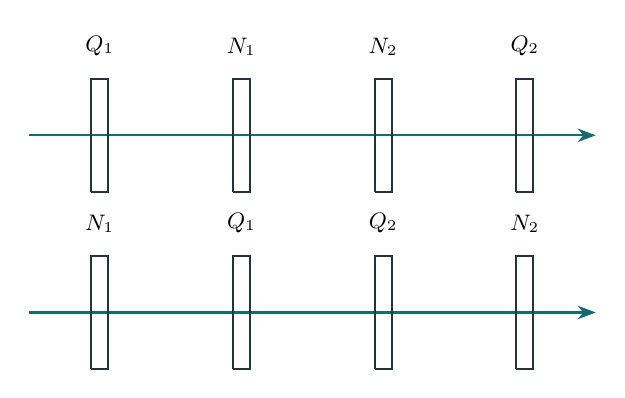
\begin{tikzpicture}[scale=.9,transform shape]
\draw[motion] (-1.00000,0.00000)--(7.00000,0.00000);\draw[object] (-0.12000,-0.80000)--(0.12000,-0.80000)--(0.12000,0.80000)--(-0.12000,0.80000)--(-0.12000,-0.80000);\node[above] at (0.00000,1.00000) {$Q_1$};\draw[object] (1.88000,-0.80000)--(2.12000,-0.80000)--(2.12000,0.80000)--(1.88000,0.80000)--(1.88000,-0.80000);\node[above] at (2.00000,1.00000) {$N_1$};\draw[object] (3.88000,-0.80000)--(4.12000,-0.80000)--(4.12000,0.80000)--(3.88000,0.80000)--(3.88000,-0.80000);\node[above] at (4.00000,1.00000) {$N_2$};\draw[object] (5.88000,-0.80000)--(6.12000,-0.80000)--(6.12000,0.80000)--(5.88000,0.80000)--(5.88000,-0.80000);\node[above] at (6.00000,1.00000) {$Q_2$};\begin{scope}[shift={(0.00000,-2.50000)}]
\draw[motion] (-1.00000,0.00000)--(7.00000,0.00000);\draw[object] (-0.12000,-0.80000)--(0.12000,-0.80000)--(0.12000,0.80000)--(-0.12000,0.80000)--(-0.12000,-0.80000);\node[above] at (0.00000,1.00000) {$N_1$};\draw[object] (1.88000,-0.80000)--(2.12000,-0.80000)--(2.12000,0.80000)--(1.88000,0.80000)--(1.88000,-0.80000);\node[above] at (2.00000,1.00000) {$Q_1$};\draw[object] (3.88000,-0.80000)--(4.12000,-0.80000)--(4.12000,0.80000)--(3.88000,0.80000)--(3.88000,-0.80000);\node[above] at (4.00000,1.00000) {$Q_2$};\draw[object] (5.88000,-0.80000)--(6.12000,-0.80000)--(6.12000,0.80000)--(5.88000,0.80000)--(5.88000,-0.80000);\node[above] at (6.00000,1.00000) {$N_2$};
\end{scope}
\end{tikzpicture}
\figcaption{图光4.15\quad 波片在两端与在两片之间的两种顺序}
\end{minipage}\end{center}

\workarea

\clearpage

\pdfbookmark[2]{第 16 题 偏振片与波片抑制镜面回光}{q16}

\section*{第 16 题\quad 偏振片与波片抑制镜面回光}\label{q:16}

自然光强度$I_0$依次通过理想偏振片、四分之一波片，正入射到理想平面镜，反射后沿同一路径返回。波片快轴与偏振片轴夹角为$\theta$。求返回并再次透过偏振片的强度，说明$\theta=45^\circ$时的结果。

\begin{center}\begin{minipage}{.98\linewidth}\centering
\begin{tikzpicture}[scale=.9,transform shape]
\draw[motion] (-1.00000,0.00000)--(5.00000,0.00000);\draw[object] (-0.12000,-0.80000)--(0.12000,-0.80000)--(0.12000,0.80000)--(-0.12000,0.80000)--(-0.12000,-0.80000);\node[above] at (0.00000,1.00000) {$P$};\node[below] at (0.00000,-1.05000) {$x$};\draw[object] (1.88000,-0.80000)--(2.12000,-0.80000)--(2.12000,0.80000)--(1.88000,0.80000)--(1.88000,-0.80000);\node[above] at (2.00000,1.00000) {$Q(\theta)$};\node[below] at (2.00000,-1.05000) {单程$\pi/2$};\draw[object] (3.88000,-0.80000)--(4.12000,-0.80000)--(4.12000,0.80000)--(3.88000,0.80000)--(3.88000,-0.80000);\node[above] at (4.00000,1.00000) {镜面};\node[below] at (4.00000,-1.05000) {法向反射};\draw[motion] (4.00000,-1.70000)--(0.00000,-1.70000);\node[below] at (2.00000,-1.80000) {沿同轴返回};
\end{tikzpicture}
\figcaption{图光4.16\quad 偏振片、波片和法向镜面的往返路径}
\end{minipage}\end{center}

\workarea

\clearpage

\pdfbookmark[2]{第 17 题 椭圆偏振光的检偏极值与主轴}{q17}

\section*{第 17 题\quad 椭圆偏振光的检偏极值与主轴}\label{q:17}

椭圆偏振光在相互垂直的$x,y$方向的分量强度为$I_x,I_y$，复振幅相对相位为$\delta$。理想检偏轴与$x$夹角为$\theta$。求透射强度、最大与最小值及相应方位，讨论退化情形。

\begin{center}\begin{minipage}{.98\linewidth}\centering
\begin{tikzpicture}[scale=.9,transform shape]
\draw[axis] (-1.50000,0.00000)--(1.50000,0.00000);\draw[axis] (0.00000,-1.50000)--(0.00000,1.50000);\node[below right] at (1.50000,0.00000) {$x$};\node[above right] at (0.00000,1.50000) {$y$};\draw[traj] plot coordinates {(0.90000,0.60000) (0.89945,0.63590) (0.89781,0.67103) (0.89507,0.70534) (0.89124,0.73879) (0.88633,0.77135) (0.88033,0.80296) (0.87327,0.83359) (0.86514,0.86321) (0.85595,0.89177) (0.84572,0.91925) (0.83447,0.94561) (0.82219,0.97082) (0.80891,0.99485) (0.79465,1.01766) (0.77942,1.03923) (0.76324,1.05954) (0.74613,1.07855) (0.72812,1.09625) (0.70921,1.11262) (0.68944,1.12763) (0.66883,1.14127) (0.64741,1.15351) (0.62519,1.16435) (0.60222,1.17378) (0.57851,1.18177) (0.55410,1.18832) (0.52901,1.19343) (0.50327,1.19708) (0.47693,1.19927) (0.45000,1.20000) (0.42252,1.19927) (0.39453,1.19708) (0.36606,1.19343) (0.33715,1.18832) (0.30782,1.18177) (0.27812,1.17378) (0.24807,1.16435) (0.21773,1.15351) (0.18712,1.14127) (0.15628,1.12763) (0.12526,1.11262) (0.09408,1.09625) (0.06278,1.07855) (0.03141,1.05954) (0.00000,1.03923) (-0.03141,1.01766) (-0.06278,0.99485) (-0.09408,0.97082) (-0.12526,0.94561) (-0.15628,0.91925) (-0.18712,0.89177) (-0.21773,0.86321) (-0.24807,0.83359) (-0.27812,0.80296) (-0.30782,0.77135) (-0.33715,0.73879) (-0.36606,0.70534) (-0.39453,0.67103) (-0.42252,0.63590) (-0.45000,0.60000) (-0.47693,0.56337) (-0.50327,0.52605) (-0.52901,0.48808) (-0.55410,0.44953) (-0.57851,0.41042) (-0.60222,0.37082) (-0.62519,0.33076) (-0.64741,0.29031) (-0.66883,0.24949) (-0.68944,0.20838) (-0.70921,0.16701) (-0.72812,0.12543) (-0.74613,0.08371) (-0.76324,0.04188) (-0.77942,-0.00000) (-0.79465,-0.04188) (-0.80891,-0.08371) (-0.82219,-0.12543) (-0.83447,-0.16701) (-0.84572,-0.20838) (-0.85595,-0.24949) (-0.86514,-0.29031) (-0.87327,-0.33076) (-0.88033,-0.37082) (-0.88633,-0.41042) (-0.89124,-0.44953) (-0.89507,-0.48808) (-0.89781,-0.52605) (-0.89945,-0.56337) (-0.90000,-0.60000) (-0.89945,-0.63590) (-0.89781,-0.67103) (-0.89507,-0.70534) (-0.89124,-0.73879) (-0.88633,-0.77135) (-0.88033,-0.80296) (-0.87327,-0.83359) (-0.86514,-0.86321) (-0.85595,-0.89177) (-0.84572,-0.91925) (-0.83447,-0.94561) (-0.82219,-0.97082) (-0.80891,-0.99485) (-0.79465,-1.01766) (-0.77942,-1.03923) (-0.76324,-1.05954) (-0.74613,-1.07855) (-0.72812,-1.09625) (-0.70921,-1.11262) (-0.68944,-1.12763) (-0.66883,-1.14127) (-0.64741,-1.15351) (-0.62519,-1.16435) (-0.60222,-1.17378) (-0.57851,-1.18177) (-0.55410,-1.18832) (-0.52901,-1.19343) (-0.50327,-1.19708) (-0.47693,-1.19927) (-0.45000,-1.20000) (-0.42252,-1.19927) (-0.39453,-1.19708) (-0.36606,-1.19343) (-0.33715,-1.18832) (-0.30782,-1.18177) (-0.27812,-1.17378) (-0.24807,-1.16435) (-0.21773,-1.15351) (-0.18712,-1.14127) (-0.15628,-1.12763) (-0.12526,-1.11262) (-0.09408,-1.09625) (-0.06278,-1.07855) (-0.03141,-1.05954) (-0.00000,-1.03923) (0.03141,-1.01766) (0.06278,-0.99485) (0.09408,-0.97082) (0.12526,-0.94561) (0.15628,-0.91925) (0.18712,-0.89177) (0.21773,-0.86321) (0.24807,-0.83359) (0.27812,-0.80296) (0.30782,-0.77135) (0.33715,-0.73879) (0.36606,-0.70534) (0.39453,-0.67103) (0.42252,-0.63590) (0.45000,-0.60000) (0.47693,-0.56337) (0.50327,-0.52605) (0.52901,-0.48808) (0.55410,-0.44953) (0.57851,-0.41042) (0.60222,-0.37082) (0.62519,-0.33076) (0.64741,-0.29031) (0.66883,-0.24949) (0.68944,-0.20838) (0.70921,-0.16701) (0.72812,-0.12543) (0.74613,-0.08371) (0.76324,-0.04188) (0.77942,-0.00000) (0.79465,0.04188) (0.80891,0.08371) (0.82219,0.12543) (0.83447,0.16701) (0.84572,0.20838) (0.85595,0.24949) (0.86514,0.29031) (0.87327,0.33076) (0.88033,0.37082) (0.88633,0.41042) (0.89124,0.44953) (0.89507,0.48808) (0.89781,0.52605) (0.89945,0.56337) (0.90000,0.60000)};\draw[traj,-{Stealth}] (0.45000,1.20000)--(0.33715,1.18832);\draw[force] (-1.23409,-0.71250)--(1.23409,0.71250);\node[above right] at (1.34667,0.77750) {检偏轴$\theta$};\node[above] at (0.00000,2.05000) {相干正交分量 $I_x,I_y,\delta$};
\end{tikzpicture}
\figcaption{图光4.17\quad 两个相干分量投影到同一检偏轴}
\end{minipage}\end{center}

\workarea

\clearpage

\pdfbookmark[2]{第 18 题 旋向不同的椭偏光通过延迟片}{q18}

\section*{第 18 题\quad 旋向不同的椭偏光通过延迟片}\label{q:18}

椭圆偏振光长短轴振幅比为2，长轴沿$y$、短轴沿$x$，总强度$I_0$。一方解石片的快轴沿$x$，使慢轴相对快轴多积累$\pi/3$相位。以$e^{-i\omega t}$约定，右、左旋入射分别写为$\sqrt{I_0/5}(1,-2i)^T$与$\sqrt{I_0/5}(1,+2i)^T$。（1）求两种入射经片后再通过方位30度检偏器的强度。（2）求各自检偏最大、最小值及方位。

\begin{center}\begin{minipage}{.98\linewidth}\centering
\begin{tikzpicture}[scale=.9,transform shape]
\draw[axis] (-1.50000,0.00000)--(1.50000,0.00000);\draw[axis] (0.00000,-1.50000)--(0.00000,1.50000);\node[below right] at (1.50000,0.00000) {$x$};\node[above right] at (0.00000,1.50000) {$y$};\draw[traj] plot coordinates {(0.75000,0.00000) (0.74954,-0.05235) (0.74817,-0.10463) (0.74589,-0.15679) (0.74270,-0.20876) (0.73861,-0.26047) (0.73361,-0.31187) (0.72772,-0.36288) (0.72095,-0.41346) (0.71329,-0.46353) (0.70477,-0.51303) (0.69539,-0.56191) (0.68516,-0.61010) (0.67410,-0.65756) (0.66221,-0.70421) (0.64952,-0.75000) (0.63604,-0.79488) (0.62178,-0.83879) (0.60676,-0.88168) (0.59101,-0.92349) (0.57453,-0.96418) (0.55736,-1.00370) (0.53950,-1.04199) (0.52099,-1.07901) (0.50185,-1.11472) (0.48209,-1.14907) (0.46175,-1.18202) (0.44084,-1.21353) (0.41939,-1.24356) (0.39744,-1.27207) (0.37500,-1.29904) (0.35210,-1.32442) (0.32878,-1.34819) (0.30505,-1.37032) (0.28095,-1.39078) (0.25652,-1.40954) (0.23176,-1.42658) (0.20673,-1.44189) (0.18144,-1.45544) (0.15593,-1.46722) (0.13024,-1.47721) (0.10438,-1.48540) (0.07840,-1.49178) (0.05232,-1.49635) (0.02617,-1.49909) (0.00000,-1.50000) (-0.02617,-1.49909) (-0.05232,-1.49635) (-0.07840,-1.49178) (-0.10438,-1.48540) (-0.13024,-1.47721) (-0.15593,-1.46722) (-0.18144,-1.45544) (-0.20673,-1.44189) (-0.23176,-1.42658) (-0.25652,-1.40954) (-0.28095,-1.39078) (-0.30505,-1.37032) (-0.32878,-1.34819) (-0.35210,-1.32442) (-0.37500,-1.29904) (-0.39744,-1.27207) (-0.41939,-1.24356) (-0.44084,-1.21353) (-0.46175,-1.18202) (-0.48209,-1.14907) (-0.50185,-1.11472) (-0.52099,-1.07901) (-0.53950,-1.04199) (-0.55736,-1.00370) (-0.57453,-0.96418) (-0.59101,-0.92349) (-0.60676,-0.88168) (-0.62178,-0.83879) (-0.63604,-0.79488) (-0.64952,-0.75000) (-0.66221,-0.70421) (-0.67410,-0.65756) (-0.68516,-0.61010) (-0.69539,-0.56191) (-0.70477,-0.51303) (-0.71329,-0.46353) (-0.72095,-0.41346) (-0.72772,-0.36288) (-0.73361,-0.31187) (-0.73861,-0.26047) (-0.74270,-0.20876) (-0.74589,-0.15679) (-0.74817,-0.10463) (-0.74954,-0.05235) (-0.75000,-0.00000) (-0.74954,0.05235) (-0.74817,0.10463) (-0.74589,0.15679) (-0.74270,0.20876) (-0.73861,0.26047) (-0.73361,0.31187) (-0.72772,0.36288) (-0.72095,0.41346) (-0.71329,0.46353) (-0.70477,0.51303) (-0.69539,0.56191) (-0.68516,0.61010) (-0.67410,0.65756) (-0.66221,0.70421) (-0.64952,0.75000) (-0.63604,0.79488) (-0.62178,0.83879) (-0.60676,0.88168) (-0.59101,0.92349) (-0.57453,0.96418) (-0.55736,1.00370) (-0.53950,1.04199) (-0.52099,1.07901) (-0.50185,1.11472) (-0.48209,1.14907) (-0.46175,1.18202) (-0.44084,1.21353) (-0.41939,1.24356) (-0.39744,1.27207) (-0.37500,1.29904) (-0.35210,1.32442) (-0.32878,1.34819) (-0.30505,1.37032) (-0.28095,1.39078) (-0.25652,1.40954) (-0.23176,1.42658) (-0.20673,1.44189) (-0.18144,1.45544) (-0.15593,1.46722) (-0.13024,1.47721) (-0.10438,1.48540) (-0.07840,1.49178) (-0.05232,1.49635) (-0.02617,1.49909) (-0.00000,1.50000) (0.02617,1.49909) (0.05232,1.49635) (0.07840,1.49178) (0.10438,1.48540) (0.13024,1.47721) (0.15593,1.46722) (0.18144,1.45544) (0.20673,1.44189) (0.23176,1.42658) (0.25652,1.40954) (0.28095,1.39078) (0.30505,1.37032) (0.32878,1.34819) (0.35210,1.32442) (0.37500,1.29904) (0.39744,1.27207) (0.41939,1.24356) (0.44084,1.21353) (0.46175,1.18202) (0.48209,1.14907) (0.50185,1.11472) (0.52099,1.07901) (0.53950,1.04199) (0.55736,1.00370) (0.57453,0.96418) (0.59101,0.92349) (0.60676,0.88168) (0.62178,0.83879) (0.63604,0.79488) (0.64952,0.75000) (0.66221,0.70421) (0.67410,0.65756) (0.68516,0.61010) (0.69539,0.56191) (0.70477,0.51303) (0.71329,0.46353) (0.72095,0.41346) (0.72772,0.36288) (0.73361,0.31187) (0.73861,0.26047) (0.74270,0.20876) (0.74589,0.15679) (0.74817,0.10463) (0.74954,0.05235) (0.75000,0.00000)};\draw[traj,-{Stealth}] (0.37500,-1.29904)--(0.28095,-1.39078);\draw[guide] (-1.42500,0.00000)--(1.42500,0.00000);\node[above right] at (1.55500,0.00000) {快轴};\node[above] at (0.00000,2.05000) {片前：长y、短x，比2:1};
\end{tikzpicture}
\figcaption{图光4.18\quad 方解石快轴对齐椭圆短轴}
\end{minipage}\end{center}

\workarea

\clearpage

\pdfbookmark[2]{第 19 题 部分椭偏光的自然分量}{q19}

\section*{第 19 题\quad 部分椭偏光的自然分量}\label{q:19}

一束沿$z$传播的单色部分椭圆偏振光，直接检偏时最大透射沿$x$且为$1.5I_0$，最小沿$y$且为$I_0$。（1）求检偏轴与$x$成任意角$\theta$时的透射强度。（2）在检偏器前插入主轴沿$x,y$的四分之一波片后，最大透射轴与$x$成30度。求插片后的最大透射强度，以及入射光中自然光部分占总强度的比例。
\begin{center}\begin{minipage}{.98\linewidth}\centering
\begin{tikzpicture}[scale=.8,transform shape]
\draw[axis] (-2,0)--(2,0) node[right] {$x$};\draw[axis] (0,-1.5)--(0,1.5) node[above] {$y$};
\node[above] at (0,2.1) {片前检偏};\node[right] at (2,0) {$1.5I_0$};\node[left] at (0,1.5) {$I_0$};
\draw[motion] (3,0)--(5,0);\node[above] at (4,.2) {四分之一波片};\node[below] at (4,-.2) {主轴沿$x,y$};
\draw[axis] (7,-1.5)--(7,1.5) node[above] {$y$};\draw[axis] (5.5,0)--(8.5,0) node[right] {$x$};\draw[force] (5.44,-.9)--(8.56,.9) node[above] {最大轴30度};
\end{tikzpicture}
\figcaption{图光4.19\quad 两次检偏的极值轴与插片条件}
\end{minipage}\end{center}

\workarea

\clearpage

\pdfbookmark[2]{第 20 题 波片产生椭圆偏振的主轴与轴比}{q20}

\section*{第 20 题\quad 波片产生椭圆偏振的主轴与轴比}\label{q:20}

振幅$A$的线偏振光与双折射片的$x$主轴夹角为$\theta$。波片使$y$相对$x$多积累相位$\delta$。推导出射椭圆的主轴方位与长短轴振幅比，并检查线偏振、圆偏振等特殊情况。

\begin{center}\begin{minipage}{.98\linewidth}\centering
\begin{tikzpicture}[scale=.9,transform shape]
\draw[axis] (-1.60000,0.00000)--(1.60000,0.00000);\draw[axis] (0.00000,-1.60000)--(0.00000,1.60000);\node[below right] at (1.60000,0.00000) {$x$};\node[above right] at (0.00000,1.60000) {$y$};\draw[motion] (-1.29904,-0.75000)--(1.29904,0.75000);\node[above right] at (1.41162,0.81500) {输入$\theta$};\node[above] at (0.00000,2.00000) {片轴$x,y$，延迟$\delta$};
\end{tikzpicture}
\figcaption{图光4.20\quad 输入线方向与晶片主轴}
\end{minipage}\end{center}

\workarea

\clearpage

\pdfbookmark[2]{第 21 题 双孔干涉中的偏振标记与检偏}{q21}

\section*{第 21 题\quad 双孔干涉中的偏振标记与检偏}\label{q:21}

自然点光源照亮杨氏双孔，两孔到屏上同一点$M$的光程差相位为$\varphi$，共同衍射包络为$D$。未放任何偏振片时，每孔单独在该点产生强度$I_0D$。起偏器$P$可放在分束前；孔后可各放$P_1,P_2$，它们的透光轴相对$P$分别为$+45^\circ,-45^\circ$；屏前还可放$P_3$。分别求：（1）仅放$P$；（2）放$P,P_1,P_2$；（3）再放与$P$平行的$P_3$；（4）把$P_3$转为与$P$垂直；（5）保持$P_1,P_2,P_3$但移去$P$。给出干涉是否存在及亮暗纹位置、峰强之间的关系。
\begin{center}\begin{minipage}{.98\linewidth}\centering
\begin{tikzpicture}[scale=.8,transform shape]
\fill (-2,0) circle(.04) node[left] {$S$};\draw[object] (0,-2)--(0,2);\draw[object] (7,-2.5)--(7,2.5) node[above] {屏};
\draw[force] (-1,-.7)--(-1,.7) node[above] {$P:x$};\fill (0,1) circle(.04) node[left] {$S_1$};\fill (0,-1) circle(.04) node[left] {$S_2$};
\draw[motion] (-2,0)--(0,1)--(7,.25);\draw[motion] (-2,0)--(0,-1)--(7,.25);\draw[force] (.5,.7)--(.5,1.3);\draw[force] (.5,-1.3)--(.5,-.7);
\node[above] at (1.5,1.5) {$P_1:+45^\circ$};\node[below] at (1.5,-1.5) {$P_2:-45^\circ$};\draw[force] (6,-1.8)--(6,1.8) node[above] {$P_3$};\fill (7,.25) circle(.04) node[right] {$M$};\node[above] at (3.9,.6) {两路相位差$\varphi$};
\end{tikzpicture}
\figcaption{图光4.21\quad 各偏振片位置及观察点$M$}
\end{minipage}\end{center}

\workarea

\clearpage

\pdfbookmark[2]{第 22 题 正交晶轴双片改变双孔条纹}{q22}

\section*{第 22 题\quad 正交晶轴双片改变双孔条纹}\label{q:22}

自然单色点光源照亮杨氏双孔。在两孔后分别插入材料、厚度$d$完全相同的双折射平行片，片面垂直光束，光轴均在片面内且互相垂直。两个主折射率为$n_o,n_e$，波长为$\lambda$。未插片时每孔在屏上贡献$I_0D$，两孔几何相位差为$\varphi$。求插片后的总强度、条纹可见度和消失条件。忽略反射、吸收及走离。

\begin{center}\begin{minipage}{.98\linewidth}\centering
\begin{tikzpicture}[scale=.8,transform shape]
\draw[object] (0,-2)--(0,2);\draw[object] (7,-2)--(7,2);\fill (0,1) circle(.04) node[left] {$S_1$};\fill (0,-1) circle(.04) node[left] {$S_2$};\draw[motion] (0,1)--(7,.3);\draw[motion] (0,-1)--(7,.3);\draw[force] (1,.5) rectangle (1.3,1.5);\draw[force] (1,-1.5) rectangle (1.3,-.5);\node[above] at (2,1.5) {$C_1:d$，轴$x$};\node[below] at (2,-1.5) {$C_2:d$，轴$y$};\node[above] at (5,1) {几何相位差$\varphi$};
\end{tikzpicture}
\figcaption{图光4.22\quad 两孔后晶片等厚，光轴互相垂直}
\end{minipage}\end{center}

\workarea

\clearpage

\pdfbookmark[2]{第 23 题 两片串联产生可调线偏方向}{q23}

\section*{第 23 题\quad 两片串联产生可调线偏方向}\label{q:23}

线偏振单色光依次通过两片相同双折射材料制成的无吸收平行片。第二片为四分之一波片，其快轴与第一片快轴夹$+45^\circ$；入射线偏方向沿第二片快轴。第一片厚度为$d$，快、慢折射率分别为$n_f,n_s$。证明出射仍为线偏振，并求其相对入射方向的有向转角。取$e^{-i\omega t}$，角度逆时针为正。

\begin{center}\begin{minipage}{.98\linewidth}\centering
\begin{tikzpicture}[scale=.9,transform shape]
\draw[motion] (-1.00000,0.00000)--(6.60000,0.00000);\draw[object] (-0.12000,-0.80000)--(0.12000,-0.80000)--(0.12000,0.80000)--(-0.12000,0.80000)--(-0.12000,-0.80000);\node[above] at (0.00000,1.00000) {输入};\node[below] at (0.00000,-1.05000) {沿$u$};\draw[object] (2.68000,-0.80000)--(2.92000,-0.80000)--(2.92000,0.80000)--(2.68000,0.80000)--(2.68000,-0.80000);\node[above] at (2.80000,1.00000) {$Q_1$};\node[below] at (2.80000,-1.05000) {快轴$x$};\draw[object] (5.48000,-0.80000)--(5.72000,-0.80000)--(5.72000,0.80000)--(5.48000,0.80000)--(5.48000,-0.80000);\node[above] at (5.60000,1.00000) {$Q_2$};\node[below] at (5.60000,-1.05000) {快轴$u=x+45^\circ$};
\end{tikzpicture}
\figcaption{图光4.23\quad 任意延迟片与45度四分之一波片}
\end{minipage}\end{center}

\workarea

\clearpage

\pdfbookmark[2]{第 24 题 白光波片的消光波长}{q24}

\section*{第 24 题\quad 白光波片的消光波长}\label{q:24}

厚度$25\,\mu\mathrm m$的方解石片放在两理想偏振片之间，片内光轴与第一片透光轴夹45度。在400至700纳米内近似取$n_o-n_e=0.172$不随波长变化。分别求两偏振片交叉、平行时不能透过的波长，并写出透射光谱因子。

\begin{center}\begin{minipage}{.98\linewidth}\centering
\begin{tikzpicture}[scale=.9,transform shape]
\draw[motion] (-1.00000,0.00000)--(5.00000,0.00000);\draw[object] (-0.12000,-0.80000)--(0.12000,-0.80000)--(0.12000,0.80000)--(-0.12000,0.80000)--(-0.12000,-0.80000);\node[above] at (0.00000,1.00000) {$P$};\node[below] at (0.00000,-1.05000) {45度分解};\draw[object] (1.88000,-0.80000)--(2.12000,-0.80000)--(2.12000,0.80000)--(1.88000,0.80000)--(1.88000,-0.80000);\node[above] at (2.00000,1.00000) {方解石};\node[below] at (2.00000,-1.05000) {$d=25\,\mu\mathrm m$};\draw[object] (3.88000,-0.80000)--(4.12000,-0.80000)--(4.12000,0.80000)--(3.88000,0.80000)--(3.88000,-0.80000);\node[above] at (4.00000,1.00000) {$A$};\node[below] at (4.00000,-1.05000) {平行或交叉};
\end{tikzpicture}
\figcaption{图光4.24\quad 白光在两偏振片与方解石片中的传播}
\end{minipage}\end{center}

\workarea

\clearpage

\pdfbookmark[2]{第 25 题 双折射劈尖的偏振干涉条纹}{q25}

\section*{第 25 题\quad 双折射劈尖的偏振干涉条纹}\label{q:25}

石英劈尖的顶角为$\alpha=30'$（30角分），钠黄光波长$589.3\,\mathrm{nm}$，$n_o=1.54424,n_e=1.55335$。劈尖置于两透光轴夹角60度的偏振片之间，晶体主轴平分此60度角。求透射光的强度随厚度的变化、条纹间距及可见度。采用薄劈尖近似，忽略反射及两分量的横向分离。

\begin{center}\begin{minipage}{.98\linewidth}\centering
\begin{tikzpicture}[scale=.9,transform shape]
\draw[object] (0.00000,0.00000)--(7.00000,0.00000)--(7.00000,1.50000)--(0.00000,0.00000);\draw[<->,thin,color=muted] (6.40000,0.00000)--(6.40000,1.37000);\node[left] at (6.40000,0.68500) {$d(x)$};\node[above] at (3.50000,1.60000) {薄劈尖：$\alpha=30^\prime$};\draw[motion] (0.00000,-0.70000)--(7.00000,-0.70000);\node[right] at (7.00000,-0.70000) {$x$};
\end{tikzpicture}
\figcaption{图光4.25\quad 劈尖的等厚线平行棱边；纵向比例示意}
\end{minipage}\end{center}

\workarea

\clearpage

\pdfbookmark[2]{第 26 题 非共线异旋圆偏振的电场干涉}{q26}

\section*{第 26 题\quad 非共线异旋圆偏振的电场干涉}\label{q:26}

两束相干的等频圆偏振平面波，在各自传播方向上旋向相反，位于$yz$平面并从$z$轴两侧以$\theta_1,\theta_2$入射到$xy$观察面。两束单独的强度标度为$I_1,I_2$。按各向同性电偶极探测的电场平方响应模型，求观察面条纹间距与可见度，讨论等强对称入射。再辨明该响应与未扰动自由场法向坡印廷通量的区别。

\begin{center}\begin{minipage}{.98\linewidth}\centering
\begin{tikzpicture}[scale=.9,transform shape]
\draw[axis] (-3.00000,0.00000)--(3.00000,0.00000);\draw[guide] (0.00000,-3.00000)--(0.00000,1.30000);\node[right] at (3.00000,0.00000) {$y$};\node[above] at (0.00000,1.30000) {$z$};\draw[motion] (1.50000,-2.50000)--(0.00000,0.00000);\draw[force] (-1.50000,-2.50000)--(0.00000,0.00000);\node[below right] at (1.50000,-2.50000) {$\hat{\boldsymbol k}_1$};\node[below left] at (-1.50000,-2.50000) {$\hat{\boldsymbol k}_2$};\node[above] at (0.00000,0.50000) {观察面$z=0$};\node[below] at (0.00000,-3.50000) {$x$垂直图面；两波各自电场垂直各自波矢};
\end{tikzpicture}
\figcaption{图光4.26\quad 非共线相反旋向圆偏波的三维几何}
\end{minipage}\end{center}

\workarea

\clearpage

\pdfbookmark[2]{第 27 题 单臂晶片对圆偏双孔条纹的作用}{q27}

\section*{第 27 题\quad 单臂晶片对圆偏双孔条纹的作用}\label{q:27}

同一圆偏振单色点光源照亮杨氏双孔，远屏满足近轴条件。在一孔后放厚度$t$的方解石平行片，片面垂直近轴光线，另一臂为空气。主折射率$n_o,n_e$，波长$\lambda$。两臂等强，忽略反射、吸收和走离。求总干涉强度、可见度，以及可见度最大、最小时的厚度。须保留晶片引起的平均相位。

\begin{center}\begin{minipage}{.98\linewidth}\centering
\begin{tikzpicture}[scale=.85,transform shape]
\fill (-3.00000,0.00000) circle(.035);\node[left] at (-3.00000,0.00000) {$S$};\draw[object] (0.00000,-2.00000)--(0.00000,2.00000);\draw[object] (7.00000,-2.50000)--(7.00000,2.50000);\node[above] at (7.00000,2.50000) {观察屏};\fill (0.00000,1.00000) circle(.035);\node[left] at (0.00000,1.00000) {$1$};\draw[motion] (-3.00000,0.00000)--(0.00000,1.00000);
\draw[motion] (0.00000,1.00000)--(7.00000,0.70000);\fill (0.00000,-1.00000) circle(.035);\node[left] at (0.00000,-1.00000) {$2$};\draw[motion] (-3.00000,0.00000)--(0.00000,-1.00000);
\draw[motion] (0.00000,-1.00000)--(7.00000,0.70000);\fill (7.00000,0.70000) circle(.035);\node[right] at (7.00000,0.70000) {$P$};\node[above] at (4.80000,1.70000) {相位差$\varphi$};\draw[very thick,color=accent] (0.70000,0.70000)--(0.70000,1.30000);\node[right] at (1.00000,1.40000) {方解石厚$t$};\node[right] at (1.00000,-1.40000) {空气};
\end{tikzpicture}
\figcaption{图光4.27\quad 圆偏双孔光在单臂加入晶片}
\end{minipage}\end{center}

\workarea

\clearpage

\pdfbookmark[2]{第 28 题 克尔盒的电压调制与条纹可见度}{q28}

\section*{第 28 题\quad 克尔盒的电压调制与条纹可见度}\label{q:28}

克尔盒长度$l=1.00\,\mathrm{cm}$，电场沿$x$，定义场致双折射为$\Delta n=K E^2$，$K=2.5\times10^{-6}\,\mathrm{m^2/V^2}$，波长$500\,\mathrm{nm}$。（1）输入为与$x$夹45度的线偏振光，出盒后用与输入正交的检偏器，求首次最强透射所需电场。（2）在等强相干双臂中分别放同样克尔盒，一盒加场$E$，另一盒不加场，输入偏振仍45度。求条纹可见度和完全显现、消失的场值。忽略损耗。

\begin{center}\begin{minipage}{.98\linewidth}\centering
\begin{tikzpicture}[scale=.9,transform shape]
\draw[motion] (-1.00000,0.00000)--(5.00000,0.00000);\draw[object] (-0.12000,-0.80000)--(0.12000,-0.80000)--(0.12000,0.80000)--(-0.12000,0.80000)--(-0.12000,-0.80000);\node[above] at (0.00000,1.00000) {45度输入};\draw[object] (1.88000,-0.80000)--(2.12000,-0.80000)--(2.12000,0.80000)--(1.88000,0.80000)--(1.88000,-0.80000);\node[above] at (2.00000,1.00000) {克尔盒};\node[below] at (2.00000,-1.05000) {$l,\ E_x$};\draw[object] (3.88000,-0.80000)--(4.12000,-0.80000)--(4.12000,0.80000)--(3.88000,0.80000)--(3.88000,-0.80000);\node[above] at (4.00000,1.00000) {交叉检偏};\node[below] at (2.00000,-1.80000) {$\Delta n=KE^2$；另以加场、无场盒比较双臂};
\end{tikzpicture}
\figcaption{图光4.28\quad 克尔延迟的强度调制与双臂比较}
\end{minipage}\end{center}

\workarea

\clearpage

\pdfbookmark[2]{第 29 题 旋光石英棱镜的圆双折射角分离}{q29}

\section*{第 29 题\quad 旋光石英棱镜的圆双折射角分离}\label{q:29}

顶角60度的旋光石英棱镜，其光轴平行棱镜底边。钠黄光处平均折射率为1.544，左、右圆偏本征波折射率差为$\Delta n=7.121\times10^{-5}$。同一平行光束以平均折射率对应的最小偏向入射角射入。在微弱圆双折射近似下，求两出射束的角分离；各本征折射率在所涉小方向范围内视为常数。

\begin{center}\begin{minipage}{.98\linewidth}\centering
\begin{tikzpicture}[scale=.8,transform shape]
\draw[object] (-1.50111,0.00000)--(0.00000,2.60000)--(1.50111,0.00000)--(-1.50111,0.00000);\draw[motion] (-2.66022,0.78910)--(-0.60000,1.56077);\node[above left] at (-2.66022,0.78910) {共同入射};\draw[motion] (-0.60000,1.56077)--(0.59999,1.56079);
\draw[motion] (0.59999,1.56079)--(3.40945,0.50866);\draw[force] (-0.60000,1.56077)--(0.60001,1.56075);
\draw[force] (0.60001,1.56075)--(3.40935,0.50832);\node[above] at (0.00000,2.80000) {$A$};\node[below] at (0.20000,-0.30000) {同一入射方向};\node[above] at (3.50000,1.20000) {两路径按Snell关系计算};
\end{tikzpicture}
\figcaption{图光4.29\quad 沿平均最小偏向路径的微弱圆双折射}
\end{minipage}\end{center}

\workarea

\clearpage

\pdfbookmark[2]{第 30 题 尼科耳棱镜的角视场}{q30}

\section*{第 30 题\quad 尼科耳棱镜的角视场}\label{q:30}

方解石尼科耳棱镜的主截面外角为68度，胶合面与入口端面垂直。光轴与入口端面夹48度。主折射率$n_o=1.658,n_e=1.486$，胶的折射率$n_g=1.550$，外部为空气。以棱镜长边方向为中央入射方向，求上下两侧允许偏离的极限，使$o$光在胶面全反射而$e$光能够透过。使用给定几何，忽略有限口径遮挡；$e$光折射必须区分波法线与能流方向。

\begin{center}\begin{minipage}{.98\linewidth}\centering
\begin{tikzpicture}[scale=.9,transform shape]
\draw[object] (0.00000,0.00000)--(0.80805,2.00000)--(6.56628,2.00000)--(5.75823,0.00000)--(0.00000,0.00000);\draw[very thick,color=accent] (0.80805,2.00000)--(5.75823,0.00000);\draw[guide] (-0.38537,2.24953)--(2.67433,1.01333);\draw[dash dot,color=muted] (0.42039,2.42916)--(1.51632,0.18217);\draw[motion] (-1.47275,1.80000)--(0.72725,1.80000);\draw[guide] (0.72725,1.80000)--(4.22725,1.80000);\node[above left] at (0.80805,2.00000) {$A$};\node[below left] at (0.00000,0.00000) {$C$};\node[below right] at (5.75823,0.00000) {$C'$};\fill (0.72725,1.80000) circle(.035);\node[below left] at (0.62725,1.60000) {$M$};\node[above] at (4.40000,1.50000) {胶面};\node[below] at (1.20000,-0.60000) {光轴};\node[above left] at (-1.20000,2.60000) {中央方向};\node[above right] at (0.45000,0.18000) {$68^\circ$};\node[below] at (3.40000,-0.40000) {光轴与端面$48^\circ$};
\end{tikzpicture}
\figcaption{图光4.30\quad 尼科耳主截面的入口、胶面与光轴}
\end{minipage}\end{center}

\workarea

\clearpage

\pdfbookmark[2]{第 31 题 波法线与能流方向的最大走离角}{q31}

\section*{第 31 题\quad 波法线与能流方向的最大走离角}\label{q:31}

单轴晶体中的$e$波，波法线与光轴夹角为$\theta$，能流方向与光轴夹角为$\xi$。求二者最大走离角，并比较方解石$n_o=1.658,n_e=1.486$与石英$n_o=1.544,n_e=1.553$的数值。

\begin{center}\begin{minipage}{.98\linewidth}\centering
\begin{tikzpicture}[scale=.9,transform shape]
\draw[axis] (-1.60000,0.00000)--(1.60000,0.00000);\draw[axis] (0.00000,-1.60000)--(0.00000,1.60000);\node[below right] at (1.60000,0.00000) {$x$};\node[above right] at (0.00000,1.60000) {$y$};\draw[guide] (-0.00000,-1.50000)--(0.00000,1.50000);\node[above left] at (0.00000,1.63000) {光轴};\draw[motion] (0.00000,0.00000)--(1.13752,1.26335);\draw[force] (0.00000,0.00000)--(1.26335,1.13752);\node[right] at (1.20000,1.70000) {$\boldsymbol k,\boldsymbol S$};\node[below] at (0.00000,-2.00000) {相位方向与能流方向分离};
\end{tikzpicture}
\figcaption{图光4.31\quad 同一e波的两种传播方向}
\end{minipage}\end{center}

\workarea

\clearpage

\pdfbookmark[2]{第 32 题 各向同性介质向晶体的全反射条件}{q32}

\section*{第 32 题\quad 各向同性介质向晶体的全反射条件}\label{q:32}

折射率$n_1$的各向同性透明介质与主折射率$n_o,n_e$的非磁单轴晶体构成平面界面。晶体光轴位于入射面，与界面法线夹$\phi$。入射线偏振的电矢量在入射面内，故激发$e$波。求发生全反射的条件与临界入射角，分别从波矢传播条件和费马原理推导。

\begin{center}\begin{minipage}{.98\linewidth}\centering
\begin{tikzpicture}[scale=.9,transform shape]
\draw[object] (-3.00000,0.00000)--(3.70000,0.00000);\draw[guide] (0.00000,-2.80000)--(0.00000,2.60000);\fill (0.00000,0.00000) circle(.035);\node[above right] at (0.00000,0.00000) {$O$};\draw[dashed,color=muted] (-1.60591,-1.78355)--(0.80296,0.89177);\node[below left] at (-1.60591,-1.78355) {光轴};\draw[motion] (-1.37658,1.96596)--(0.00000,0.00000);\draw[motion] (0.00000,0.00000)--(0.98477,-2.40629);\node[below left] at (0.98477,-2.40629) {$\boldsymbol k_t$};\draw[force] (0.00000,0.00000)--(1.35387,-2.67713);\node[below right] at (1.35387,-2.67713) {$\boldsymbol S_t$};\node[right] at (-2.70000,1.40000) {$n_1$};\node[right] at (2.50000,-1.00000) {晶体};\node[above] at (2.00000,2.40000) {入射p偏振};
\end{tikzpicture}
\figcaption{图光4.32\quad 主截面内从外介质进入晶体}
\end{minipage}\end{center}

\workarea

\clearpage

\pdfbookmark[2]{第 33 题 晶体内反射的光线角关系}{q33}

\section*{第 33 题\quad 晶体内反射的光线角关系}\label{q:33}

单轴晶体内的$e$光线在平面界面反射，光轴在主截面内，与指向晶体内部的法线夹$\phi$。求入射、反射能流角之间的关系，说明为何它们一般不相等。给出波矢法与费马法，并正确选择反射分支。只讨论同一$e$本征通道。

\begin{center}\begin{minipage}{.98\linewidth}\centering
\begin{tikzpicture}[scale=.9,transform shape]
\draw[object] (-3.50000,0.00000)--(3.50000,0.00000);\draw[guide] (0.00000,-3.00000)--(0.00000,1.00000);\draw[force] (-1.50000,-2.59808)--(0.00000,0.00000);
\draw[force] (0.00000,0.00000)--(1.86955,-2.34623);\node[below left] at (-1.50000,-2.59808) {入射能流};\node[below right] at (1.86955,-2.34623) {反射能流};\draw[guide] (-1.80665,-2.00649)--(0.66913,0.74314);\draw[thin,color=muted] (-1.80665,-2.00649)--(-3.00000,-0.90000);\node[left] at (-3.00000,-0.90000) {光轴};
\end{tikzpicture}
\figcaption{图光4.33\quad 晶体内部反射的入射与出射能流}
\end{minipage}\end{center}

\workarea

\clearpage

\pdfbookmark[2]{第 34 题 晶体界面的振幅反射与透射}{q34}

\section*{第 34 题\quad 晶体界面的振幅反射与透射}\label{q:34}

折射率$n_1$的各向同性透明非磁介质向主折射率$n_o,n_e$的透明非磁单轴晶体入射$p$线偏振光，光轴在入射主截面内，与法线夹$\phi$。推导电场总振幅反射系数$r$与透射系数$t$。应明确晶内波法线角$\theta_p$、能流角$\theta_t$及方向折射率$n_p$怎样确定，并给出法向入射结果和法向能流的守恒关系。

\begin{center}\begin{minipage}{.98\linewidth}\centering
\begin{tikzpicture}[scale=.9,transform shape]
\draw[object] (-3.00000,0.00000)--(3.70000,0.00000);\draw[guide] (0.00000,-2.80000)--(0.00000,2.60000);\fill (0.00000,0.00000) circle(.035);\node[above right] at (0.00000,0.00000) {$O$};\draw[dashed,color=muted] (-1.60591,-1.78355)--(0.80296,0.89177);\node[below left] at (-1.60591,-1.78355) {光轴};\draw[motion] (-1.37658,1.96596)--(0.00000,0.00000);\draw[motion] (0.00000,0.00000)--(0.98477,-2.40629);\node[below left] at (0.98477,-2.40629) {$\boldsymbol k_t$};\draw[force] (0.00000,0.00000)--(1.35387,-2.67713);\node[below right] at (1.35387,-2.67713) {$\boldsymbol S_t$};\node[right] at (-2.70000,1.40000) {$n_1$};\node[right] at (2.50000,-1.00000) {晶体};\draw[motion] (0.00000,0.00000)--(1.37658,1.96596);\node[right] at (1.37658,1.96596) {反射};
\end{tikzpicture}
\figcaption{图光4.34\quad p偏振入射、晶内波法线与能流}
\end{minipage}\end{center}

\workarea

\clearpage

\pdfbookmark[2]{第 35 题 晶体界面的可逆路径与斯托克斯关系}{q35}

\section*{第 35 题\quad 晶体界面的可逆路径与斯托克斯关系}\label{q:35}

对各向同性透明介质与单轴透明晶体的主截面$p$偏振界面，证明传播路径的可逆性，并由逆向场叠加推导振幅反射、透射系数的斯托克斯关系。晶内反射光线一般不等角，需区分沿透射束反向入射与沿外侧反射束反向入射两种实验。各介质无吸收、互易，所有相关支均为传播波。

\begin{center}\begin{minipage}{.98\linewidth}\centering
\begin{tikzpicture}[scale=.9,transform shape]
\draw[object] (-2.20000,0.00000)--(2.20000,0.00000);\draw[guide] (0.00000,-2.20000)--(0.00000,2.00000);\draw[motion] (-1.80000,1.70000)--(0.00000,0.00000);
\draw[motion] (0.00000,0.00000)--(1.80000,1.70000);\draw[force] (0.00000,0.00000)--(0.90000,-2.00000);\node[above] at (-1.80000,1.70000) {$A$};\node[above] at (1.80000,1.70000) {$Ar$};\node[below] at (0.90000,-2.00000) {$At$};\node[above] at (0.00000,2.60000) {正向分束：外侧反射与晶内透射};
\end{tikzpicture}
\figcaption{图光4.35\quad 正向传播的两条出射路径}
\end{minipage}\end{center}

\workarea

\end{document}
